\documentclass[10pt,letterpaper]{article}

\usepackage{cvpr}
\usepackage{times}
\usepackage{epsfig}
\usepackage{graphicx}
\usepackage{amsmath}
\usepackage{amssymb}
\usepackage{algorithm}
\usepackage{algorithmic}
\usepackage{etoolbox}\AtBeginEnvironment{algorithmic}{\footnotesize}

% Include other packages here, before hyperref.

% If you comment hyperref and then uncomment it, you should delete
% egpaper.aux before re-running latex.  (Or just hit 'q' on the first latex
% run, let it finish, and you should be clear).
\usepackage[breaklinks=true,bookmarks=false]{hyperref}

\cvprfinalcopy % *** Uncomment this line for the final submission

\def\cvprPaperID{****} % *** Enter the CVPR Paper ID here
\def\httilde{\mbox{\tt\raisebox{-.5ex}{\symbol{126}}}}

% Pages are numbered in submission mode, and unnumbered in camera-ready
%\ifcvprfinal\pagestyle{empty}\fi
\setcounter{page}{1}
\begin{document}

%%%%%%%%% TITLE
\title{A Parallelized Framework for Evolutionary Computation}

\author{
	Geoffrey Saxton Long (\textit{260403840})\\
	McGill University, Quebec \\
	{\tt\small Geoffrey.Long@mail.mcgill.ca}
}

\maketitle
%\thispagestyle{empty}

%%%%%%%%% ABSTRACT
\begin{abstract}
Evolutionary algorithms are a common approach to problems with indeterminate strategies or lengthy computation times when exact results are not necessary. The goal of this project is to implement an extensible framework which allows for parallelization of an evolutionary algorithm. Although computation speed is a primary goal, I would also like to see the outcomes where "populations" of individuals are allowed to evolve in partial, or complete, isolation from one another. Each one of these populations would be implemented on a multithreaded Beowulf cluster, exposure to other populations would occur via MPI message passing. Within each cluster the populations would be evolved through different mutation, crossover, and fitness evaluation methods. This variance in operators would ensure that the populations diverge. 

This framework will implement a genetic algorithm. Although the algorithm will be tested with the Travelling Salesperson Algorithm, it will be designed to work with a wide variety of problems. The overall performance of the framework will be evaluated on the results and speedup compared to the sequential version. 
\end{abstract}

% http://watchmaker.uncommons.org/manual/ch01s02.html
% EC is good for problems where you know what comprises a good solution, but you don't necessarily know how to reach this solution. 


\section{Introduction}
Evolutionary Computation is a branch of computational intelligence commonly used to solve problems with complex relationships between the parameters, multiple local optima, or no known approach to solving the problem. The term Evolutionary computation covers several different algorithmic approaches. These are evolutionary programming, genetic programming, genetic algorithms, and evolution strategies. Although the approaches to each of these frameworks is slightly different, they all have the same general structure and themes; specifically, the adherance to Darwinian principles. 

The darwinian principles central to evolutionary computation are those of evolution by natural selection. This is commonly broken into four main themes:
\begin{enumerate}
\item More individuals are produced each generation than can survive
\item Variation exists amoung individuals, this variation is inhertiable
\item Those individuals with inherited traits better suited to the environment will survive
\item When reproductive isolation occurs a new species will form
\end{enumerate}

%TODO in order to make this simpler could talk about it in terms of TSP

The above can be abstracted easily into programming. To model evolution in a compter environment you need a few data pieces and operators. Central to evolutionary computation is the \textit{population}. This population is a set of \textit{individuals}, which are each an encoding of a possible solution. The individuals can be analyzed on how well they solve the underlying problem. This analysis is called \textit{fitness evaluation} and the score attributed to each individual is called its \textit{fitness}.

Commonly these individuals are bit strings, however they can have more complex structures. The way in which the individual (solution) is encoded is often unique to the problem and specific implementation. The individual can be optimized to be space efficient, easily manipulated, or easily understood. However the solution is constructed, it will only be successful if it can be changed by the evolutionary operators in the framework. 

The evolutionary operators most commonly used are \textit{mutation} and \textit{crossover}. Although mutation is present in all evolutionary computation methods, crossover is often specific to certain subsets of evolutionary computation such as genetic algorithms. Both of these operators act on \textit{alleles}, which are the smallest differentiable part of each individual. % Differentiable isn't really the right word, more like the smallest unit that can stand alone, or the smallest that can have a healthy abstraction

Mutation is the alteration of an individual via a slight change in their genetic makeup. This change typically occurs through altering one of the individual's alleles or by switching two or more alleles. The resultant individual is slightly different than the original. The implementation determines how slight this difference is.

Crossover involves the creation of a new individual by combining two or more "parent" individuals. Typically, these parents are selected based on their genetic fitness. The fittest individuals are usually the ones allowed to procreate. When the parents are selected, the crossover operators usually use sections of each to create one or more new individuals.  


%survival of the fittest (natural selection), mutation, mating, 
%As the name suggests, Evolutionary Computation methods follow the common themes of evolution as described by Darwin. 



\section{Background}
% Previous algorithms, previous attempts at parallelization?


\section{Implementation}
\subsection{v1.1}
The first iteration of the genetic algorithm framework was a simple mutation and fitness based selection algorithm. Each individual was mutated via a swap (where two cities in the tour were switched at random) too create a new individual. The fitter of the two was chosen for the next generation. Since there was no crossover, this implementation was more of an evolutionary programming method. 
%Each parent generates its own offspring. The parent is then compared to it's offspring, and the fitter of the two is allowed to survive. 

The purpose of this version was to characterize the relationships between the various parameters. The parameters compared in this phase were the number of threads, the population size, and the number of iterations. These parameters were evaluated as per their impact on the fitness score of the fittest individual and execution time. The goal was to find relationships between these parameters. By finding relationships, futher testing could be constrained by focusing on only the most important parameters. 

The first tests were focused on analyzing how fitness varied with the parameters. The first parameter focused on was the number of threads. Since the number of threads does not change the underlying computations, the fitness should be unaffected by an increase in the thread count. By manual inspection of the data, this was shown to be true. Since these two are uncorrelated, the fitness score of individuals can be largely left out when discussing the efficacy of the parallel implementation. It was also found that while an increase in population size does improve the fitness of the individual, there is a larger increase in fitness when the number of iterations is bolstered.

Since fitness proved to be rather irrelavent in discussion of the parallel performance, speedup and execution time were focused on next. An almost linear relationship was found between the parameters population size and number of iterations (taken individually) and execution time. Doubling either the maximum number of iterations or the population size almost doubles the execution time. Therefore, population size and number of iterations seem to be directly proportional in their effect on execution time.

Since we can take the population size and number of iterations to be roughly equal in their implact on execution time, we can view how varying the thread count will impact both. This involved graphical analysis of the relative execution times where population size and number of iterations were varied independently over a range of thread counts. From the graph %TODO ref
, it can be seen that the number of threads impact both the same. So, when the number of iterations and the population size are both much greater than the number of threads, a change in the population size or the number of iterations will have generally the same effect on speedup.

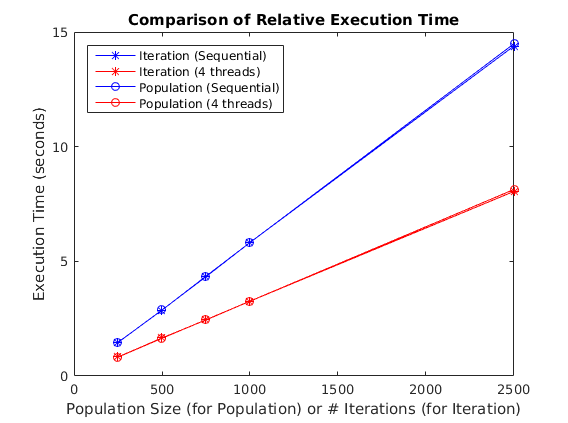
\includegraphics[scale=1]{../img/Lenovo_Compare_ItervsPop.png} 

This relationship only holds for small thread counts though. As the number of threads approaches the population size, the speedup decreases quickly. This is shown by the graphs of population size vs thread count. %TODO refs
Although this relationship exists between population size and speedup, there doesn't appear to be any relationship between number of iterations, number of threads, and speedup. This is shown by the graphs in Figure %TODO refs
The reason why the population size has such a large effect is due to how the algorithm is parallelized. The OpenMP parallel construct was placed around a loop over the individuals in a population. When the number of threads increases, each thread is responsible for fewer and fewer individuals. When the number of threads is equal to the population size, each thread is responsible for one loop over one individual. The cost of spawning a thread is great when compared to the relatively small amount of work the thread is responsible for. An anomaly worth noting is that for 24 threads, the Debondt system has no speedup at all. %TODO explain this please


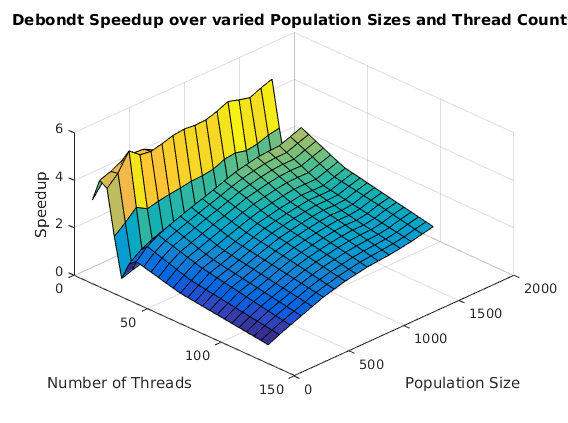
\includegraphics[scale=1]{../img/Debondt_PopulationvsThreads.png} 
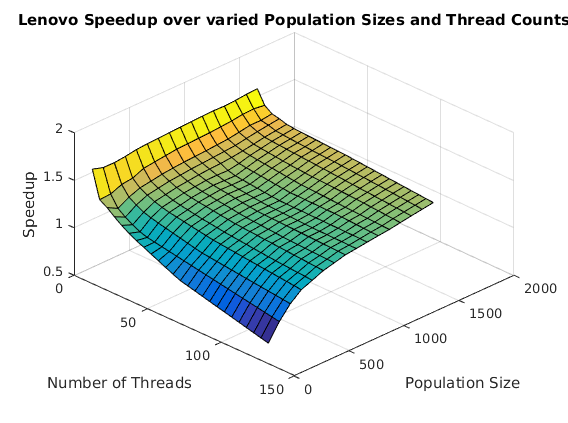
\includegraphics[scale=1]{../img/Lenovo_PopulationvsThreads.png} 


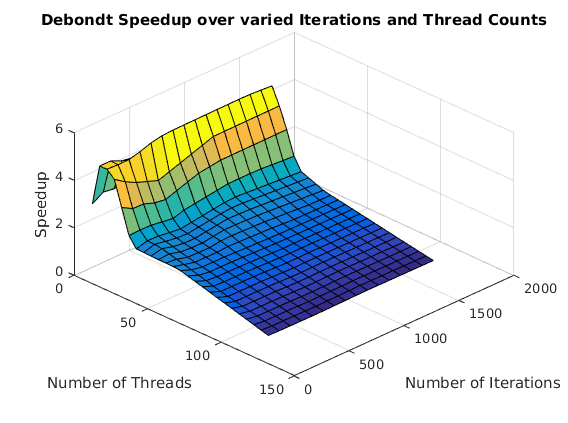
\includegraphics[scale=1]{../img/Debondt_IterationvsThreads.png} 
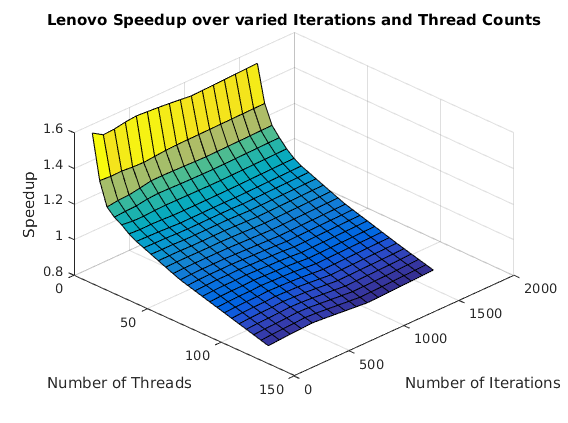
\includegraphics[scale=1]{../img/Lenovo_IterationvsThreads.png} 


So, based on the above, if the population size is sufficiently high, the population size and iteration count can essentially be left out of conversations on speedup. In order to accuratly calculate speedup, an ideal number for population size and maximum number of iterations was ascertained. This was found by running the program on the Lenovo with a set number of threads and a varying population size and iteration number. From the resultant graph (Figure %TODO ref
), I found that a population size of 500 with an iteration number of 10000 was ideal for futher testing. These number maximized the speedup and minimized the overall execution time while still providing a good final fitness. 

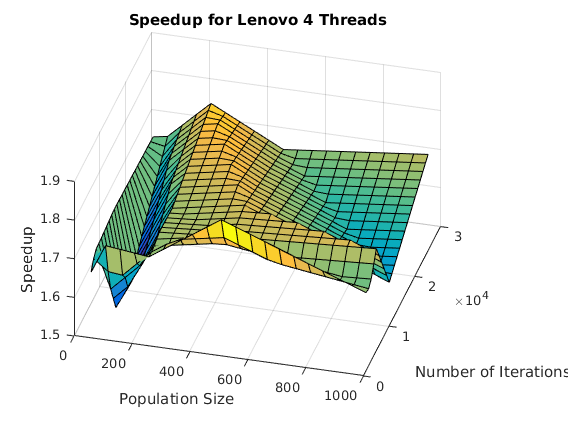
\includegraphics[scale=1]{../img/Lenovo_4Thread_PopvsIter.png} 

When running the algorithm on the EIL51 dataset with the aforementioned sizes, I get a maximum speedup of 1.75 on a Lenovo ideapad with an Intel(R) Core(TM) i5-4200U CPU @ 1.60GHz. This processor has two cores with two threads per core. With hyperthreading this creates four virtual cores. The peak speedup occurs at 2 threads, and again at 4 threads. Three threads sees a bit of a lull. This may be because of OpenMP's thread migration. Two threads is really all the computer can fully utilize though, since hyperthreading doesn't really help for cases such as this where there is a lot of floating point computation. %TODO see when hyperthreading does work %TODO link to convo about 24 threads in Debondt

Since only having two cores was severly limiting, I got access to a cim server called Debondt. This server has %TODO list out specs. 

Armed with Debondt, I was able to then do some testing in parallel, which sped up my results acquisition phase. The aforementioned sizes were then run on Debondt and the Lenovo with variable thread counts to characterize the speedup. From these trials I got the following graphs. 

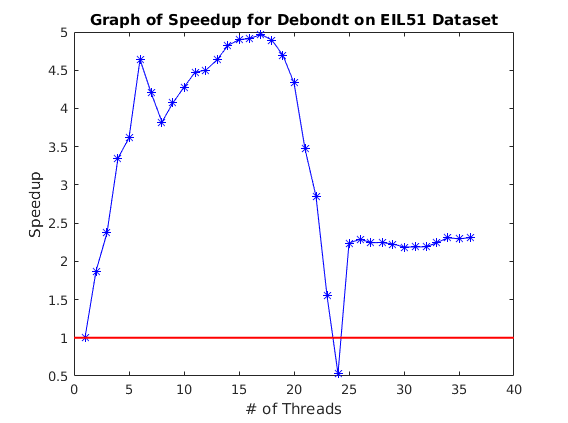
\includegraphics[scale=1]{../img/Debondt_speedup.png} 
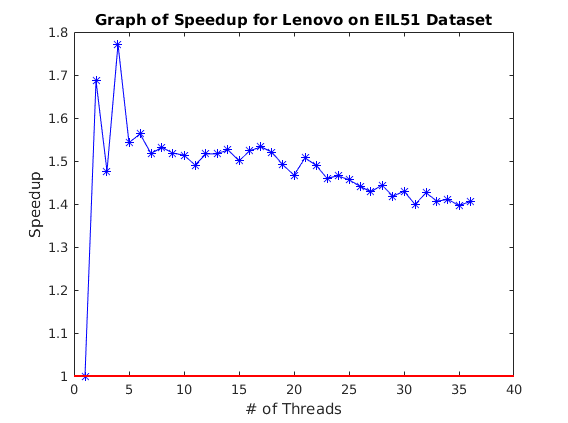
\includegraphics[scale=1]{../img/Lenovo_Speedup.png} 


The final trials involved determining the effects of tour size on the speedup. Thankfully, I had a few different tours of varied length. These were run using Debondt and the outcome was graphed in Figure %TODO ref

%TODO add graph of different tour stuff


%If we follow the fastest runtimes, then both the PThreads and OpenMP programs reach their peak performance at four threads. My computer is running an Intel(R) Core(TM) i5-4200U CPU @ 1.60GHz. This processor has two cores with two threads per core. With hyperthreading this creates four virtual cores. It then makes sense that the fastest runtimes would appear at four threads, since four threads is the maximum number of "simultaneous" (due to hyperthreading) threads that can be run. At any number less than four threads, the program isn't harnessing all of the computer resources. Anything over four threads and the threads will be interleaved. % Get better word
%Theoretically, having more threads than cores could be advantageous if any threads have to wait for I/O or mutex variables. In this case, the threads would run on the CPU cycles when the other threads are waiting. In this program, however, the processing component is not too intensive compared to the I/O requirements and therefore having more threads than the number of cores provides no notable benefits. As a matter of fact, these instances with large thread counts actually will run slower since each thread will take a non-trivial amount of time to instantiate each thread.

%Although the fastest runtimes occur at a thread count of four for PThreads and OpenMP run, OpenMP generally runs faster at eight cores. This may have to do with OpenMP's thread migration and CPU affinity settings. When the number of threads exceeds the number of cores, then the threads of OpenMP may optimally migrate from core to core. When the number of threads matches the number of cores, however, the thread is likely locked to the virtual core. Since this core is only virtual, if a single thread is pushing the physical core to 100\% usage then this may be consuming both virtual cores. This would explain the strange values in OpenMP when the number of threads is four. It does not explain why the binarized version performed so much worse than the Sobel version for four threads. Perhaps this has to do with the dynamic runtime environment of OpenMP and how cores are bound at runtime. Further testing would involve changing more of the environment variables, such as OMP\_PROC\_BIND and GOMP\_CPU\_Affinity, as well as testing with pixel padding. I did try altering the loops indexing; running the OpenMP in their double for loop (instead of flattening) with collapse(2); and running the loops with slightly different OpenMP commands (such as schedule(dynamic) with different chunk sizes). None of these offered a performance increase though, nor did they change the strange behaviours I referenced earlier.



\subsection{v1.2}
In this version, additional mutation operators were added as well as a crossover and parent selection technique.


\section{Results}

\section{Conclusions}


\section{Pertinent Results}
\subsection{Simple Sequential}
\subsubsection{Population Based}
PopulationSize=100 maxNumIterations=100 Fitness=1006.61 Time=0.0594495
PopulationSize=200 maxNumIterations=100 Fitness=971.531 Time=0.116636
PopulationSize=300 maxNumIterations=100 Fitness=983.57 Time=0.179451
PopulationSize=400 maxNumIterations=100 Fitness=940.753 Time=0.23334
PopulationSize=500 maxNumIterations=100 Fitness=985.453 Time=0.292069
PopulationSize=600 maxNumIterations=100 Fitness=995.133 Time=0.353345
PopulationSize=700 maxNumIterations=100 Fitness=976.031 Time=0.438044
PopulationSize=800 maxNumIterations=100 Fitness=959.766 Time=0.466137
PopulationSize=900 maxNumIterations=100 Fitness=969.391 Time=0.522619
PopulationSize=1000 maxNumIterations=100 Fitness=972.207 Time=0.585324
PopulationSize=2000 maxNumIterations=100 Fitness=942.047 Time=1.17845
PopulationSize=3000 maxNumIterations=100 Fitness=938.467 Time=1.88575
PopulationSize=4000 maxNumIterations=100 Fitness=940.066 Time=2.37096
PopulationSize=5000 maxNumIterations=100 Fitness=927.209 Time=3.02321
PopulationSize=6000 maxNumIterations=100 Fitness=920.407 Time=3.73201
PopulationSize=7000 maxNumIterations=100 Fitness=919.812 Time=4.54565
PopulationSize=8000 maxNumIterations=100 Fitness=922.916 Time=5.10203
PopulationSize=9000 maxNumIterations=100 Fitness=929.764 Time=5.55095
PopulationSize=10000 maxNumIterations=100 Fitness=925.476 Time=6.07093

\subsubsection{Iteration Based}
PopulationSize=100 maxNumIterations=100 Fitness=1005.18 Time=0.0612377
PopulationSize=100 maxNumIterations=200 Fitness=879.523 Time=0.117883
PopulationSize=100 maxNumIterations=300 Fitness=800.886 Time=0.174866
PopulationSize=100 maxNumIterations=400 Fitness=791.031 Time=0.237152
PopulationSize=100 maxNumIterations=500 Fitness=716.329 Time=0.292422
PopulationSize=100 maxNumIterations=600 Fitness=700.984 Time=0.351435
PopulationSize=100 maxNumIterations=700 Fitness=698.819 Time=0.41049
PopulationSize=100 maxNumIterations=800 Fitness=685.63 Time=0.476722
PopulationSize=100 maxNumIterations=900 Fitness=667.82 Time=0.530665
PopulationSize=100 maxNumIterations=1000 Fitness=650.368 Time=0.59416
PopulationSize=100 maxNumIterations=2000 Fitness=573.286 Time=1.23812
PopulationSize=100 maxNumIterations=3000 Fitness=534.997 Time=1.79002
PopulationSize=100 maxNumIterations=4000 Fitness=521.264 Time=2.36564
PopulationSize=100 maxNumIterations=5000 Fitness=510.855 Time=2.95029
PopulationSize=100 maxNumIterations=6000 Fitness=503.941 Time=3.781
PopulationSize=100 maxNumIterations=7000 Fitness=505.155 Time=4.3372
PopulationSize=100 maxNumIterations=8000 Fitness=498.558 Time=4.94316
PopulationSize=100 maxNumIterations=9000 Fitness=502.808 Time=5.59283
PopulationSize=100 maxNumIterations=10000 Fitness=497.015 Time=6.0404

\subsubsection{Thread Based}
Threads=1 PopulationSize=500 maxNumIterations=10000 Fitness=480.492 Time=28.9301
Threads=2 PopulationSize=500 maxNumIterations=10000 Fitness=481.042 Time=17.08
Threads=3 PopulationSize=500 maxNumIterations=10000 Fitness=486.164 Time=19.4246
Threads=4 PopulationSize=500 maxNumIterations=10000 Fitness=481.419 Time=16.1616
Threads=6 PopulationSize=500 maxNumIterations=10000 Fitness=478.596 Time=18.4624
Threads=8 PopulationSize=500 maxNumIterations=10000 Fitness=484.597 Time=18.7737
Threads=16 PopulationSize=500 maxNumIterations=10000 Fitness=484.133 Time=19.2235
Threads=32 PopulationSize=500 maxNumIterations=10000 Fitness=485.378 Time=20.5241
Threads=64 PopulationSize=500 maxNumIterations=10000 Fitness=480.417 Time=20.9859








\section{Sources}
% http://courses.cs.washington.edu/courses/cse466/05sp/pdfs/lectures/10-EvolutionaryComputation.pdf
% http://evolution.berkeley.edu/evolibrary/article/evo_25
% https://www.ndsu.edu/pubweb/~mcclean/plsc431/popgen/popgen5.htm
% http://comopt.ifi.uni-heidelberg.de/software/TSPLIB95/
%	Used the symmetric TSP stuff


\end{document}